\documentclass[a4paper,12pt] {article}
\usepackage {color}
\usepackage{graphicx} 
\usepackage{indentfirst}
\usepackage{enumerate}

\title{Rangkuman Basis Data Pertemuan ke-3}
\author{}
\date{}

\begin{document}
\begin{titlepage}
\maketitle
\thispagestyle{empty}

\vspace{0.5cm}
\begin{center}

\includegraphics[width=8.5cm, height=8cm]{poltekpos.png}
\end{center}
\vspace{0.5cm}
\begin{center}
Diajukan untuk memenuhi tugas mata kuliah Basis Data\\
\vspace{12px}
Dosen Pengampu:\\
Syafrial Fachri Pane, ST., MTI., EBDP.
\vspace{12px}

Oleh:\\
Muhammad Fahri Ramadhan\\
1194055
\vspace{14px}

\textbf{PROGRAM DIPLOMA IV TEKNIK INFORMATIKA}\\
\textbf{POLITEKNIK POS INDONESIA\\}\textbf{BANDUNG}\\
\textbf{2020}
\end{center}
\end{titlepage}


\newpage

\maketitle


\section{Pengertian Basis Data}
 Basis data terdiri dari dua terdiri dari dua kata yaitu, basis yang berarti gudang, markas, atau tempat penyimpanan, dan data yang berarti sebuah nilai yang merepresentasikan objek atau kejadian di dunia nyata
\par Secara istilah, basis data dapat dikatakan sebagai suatu himpunan data yang berhubungan satu sama lain dan tanpa pengulangan. Basis data disimpan dalam perangkat elektronik, lalu diorganisasikan agar dapat dimanfaatkan dengan cepat dan mudah.
Basis data haruslah diterapkan pada zaman ini, karena data adalah suatu hal yang sangat penting bagi kehidupan manusia. Data menjadi sebuah referensi atau patokan untuk berbagai hal, contohnya saja dalam mengembangkan teknologi maka dibutuhkan data untuk membuat teknologi terbarukan.

\section{Tujuan Basis Data}
\subsection{Kecepatan (Speed)}
Pada basis data, proses create, update, delete menjadi lebih cepat.
\subsection{Ruang Penyimpanan(Space)}
Pada basis data ruang penyimpanan bisa ditekan seminimal mungkin karena tidak akan terjadi redudansi dan juga tabel yang saling berhubungan membuat ruang penyimpanan menjadi efisien.
\subsection{Ketepatan (Accuracy)}
Pada basis data diterapkan sistem primary key, yang membuat ketepatan sebuah data terjamin.


\section{Macam-macam Basis Data}
\subsection{SQL}
Merupakan basis data relasional yaitu atribut yang awalnya berada pada satu tabel dikumpulkan, lalu diorganisasikan, dinormalisasi, dan terbentuklah beberapa tabel, lalu tabel tersebut direlasikan.
\subsection{No-SQL}
Merupakan basis data yang semua atributnya berada pada satu tabel dan tidak melewati tahapan lainnya.

\section{Macam-macam Kunci(Key)}
Untuk merelasikan tabel satu dengan tabel lainnya, dibutuhkan atribut yang unik pada tiap-tiap tabelnya. Dalam basis data terdapat jenis kunci yaitu:
\subsection{Super Key}
Pada data/semua tabel yang dikumpulkan terdapat  beberapa atribut yang bersifat unik, atribut tersebut adalah super key
\subsection{Candidate Key}
Dalam satu tabel terdapat beberapa atribut yang bersifat unik, atribut tersebut dapat dikatakan sebagai candidate key
\subsection{Primary Key}
Candidate key yang terpilih untuk mewakili suatu tabel sebagai kode unik dinamakan primary key.
\subsection{Foreign Key}
Tabel lain berelasi dengan sebuah tabel, maka primary key pada tabel lain menjadi foreign key pada tabel yang direlasikan.

\section{Pangkat Kardinalitas}
Agar dapat merelasikan tabel satu dengan lainnya maka dibutuhkan pengetahuan mengenai pangkat kardinalitas. Terdapat beberapa pangkat kardinalitas yaitu:
\begin{itemize}
\item One to one relationship
\item One to many relationship
\item Many to one relationship
\item Many to many relationship
\end{itemize}

\section{Perbedaan CDM dan PDM}
Proses normalisasi harus melalui beberapa tahapan, pada tahapan-tahapan tersebut tabel yang dinormalisasi harus melalui tahap CDM dan PDM terlebih dahulu. Berikut penjelasan singkat mengenai perbedaan antara CDM dan PDM.
\par CDM bisa dikatakan sebagai pengelompokan data dan hanya ada garis relasi tanpa adanya arah pada garis relasi tersebut. Sedangkan PDM adalah penggambaran basis data yang sesungguhnya, sudah terdapat primary key, juga arah relasi dari tabel satu ke tabel lainnya.

\section{Tugas Membuat CDM dan PDM Absensi Mahasiswa}
\subsection{CDM Absensi Mahasiswa}
\vspace{0.5cm}
\begin{center}
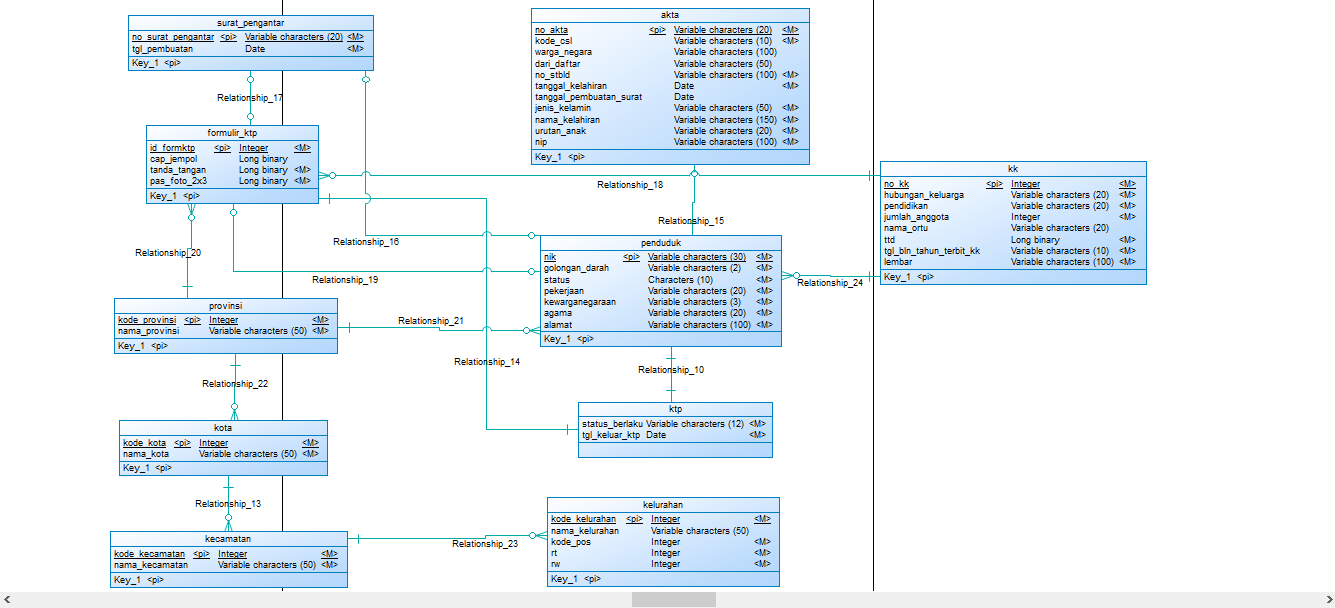
\includegraphics[width=8.5cm, height=8cm]{cdm.png}
\end{center}
\vspace{0.5cm}
\par Pada CDM terlihat bahwa atribut-atribut dikelompokan, lalu direlasikan satu sama lain. Pada tabel CDM ini belum ditentukan primary key pada tiap-tiap tabelnya dan juga kita belum mengetahui arah garis relasinya.
\subsection{PDM Absensi Mahasiswa}
\vspace{0.5cm}
\begin{center}
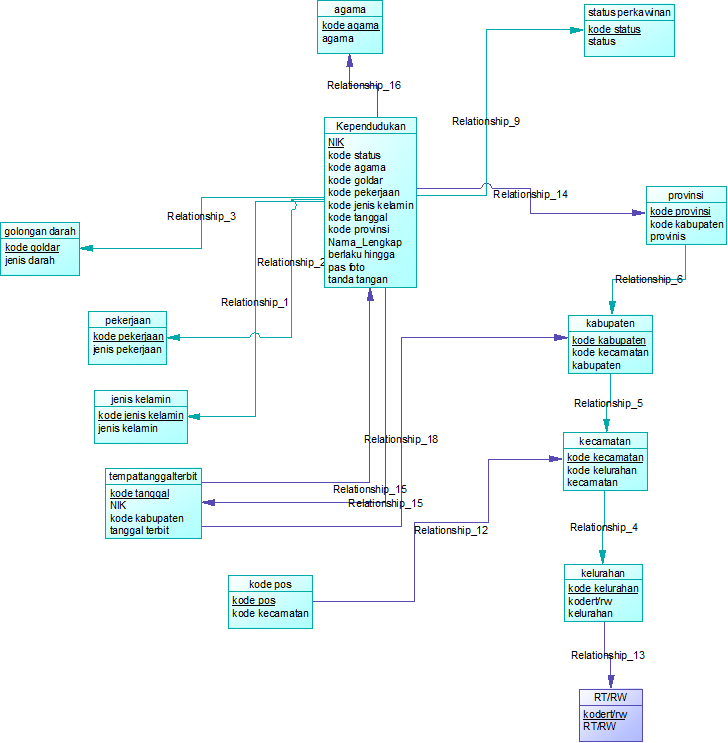
\includegraphics[width=8.5cm, height=8cm]{pdm.png}
\end{center}
\vspace{0.5cm}
\par Setelah melewati CDM, maka kita dapat menentukan tabel yang menjadi master. Tabel Jadwal merupakan tabel master, karena tiap-tiap tabel berelasi menuju Tabel Jadwal. Pada tahap PDM juga primary key pada tiap-tiap tabel telah ditentukan begitu pula arah garis relasinya sudah jelas.
\par Tabel Jadwal berelasi dengan tiga tabel yaitu:
\begin{itemize}
\item Tabel mata kuliah yang memiliki primary key berupa kode mata kuliah dan menjadi foreign key saat direlasikan dengan tabel jadwal
\item Tabel mahasiswa yang memiliki primary key berupa NPM dan menjadi foreign key saat direlasikan dengan tabel jadwal
\item Tabel pegawai yang memiliki primary key berupa NIK dan menjadi foreign key saat direlasikan dengan tabel jadwal
\end{itemize}
\par Setelah tabel-tabel lainnya direlasikan, maka tabel jadwal harus mempunyai primary key juga. Pada tabel master, primary key biasanya berupa id\_nama-tabel dan biasanya nilai primary key tersebut auto increment.

\end{document}